%!TEX root = ./lec03_hardware.tex


%
% ---------------------------------------------------------------------------
%
\begin{frame}{Database \textbf{Application} Architecture}

Multi-user applications are best developed as client-server applications.

\begin{block}{\alert{Client-Server} applications}
The DBMS (server) and the application (client) run as independent processes, often on different computers. There usually is one server for many clients.
\end{block}

\vskip1em

Single-user applications (e.g., apps on mobile devices or some games) can be developed as a single process:

\begin{block}{\alert{Embedded DBMS} applications}
The application and the DBMS are \textbf{compiled} together and run as a single process on the same device.
\end{block}


\end{frame}

%
% ---------------------------------------------------------------------------
%
\begin{frame}
\label{client_server_separate}
\textbf{Client-server} on separate computers:

\begin{center}
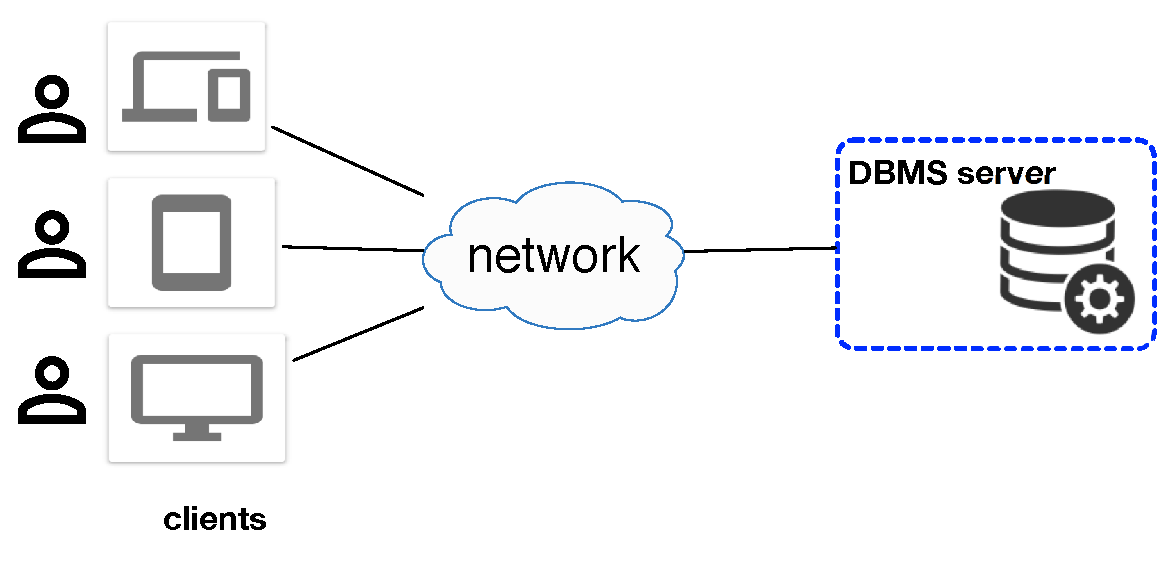
\includegraphics[width=0.75\textwidth]{figures/client_server_cloud}
\end{center}

\textbf{Example: Beartracks} (clients are Web apps on browsers)

\begin{BOX}{Connecting to the server}
The client needs a \emph{connector} API to talk to the DBMS.

\vskip0.5em

ODBC\footnotemark  is widely used for this.
\end{BOX}

\footnotetext{\url{https://en.wikipedia.org/wiki/Open_Database_Connectivity}}
\end{frame}

%
% ---------------------------------------------------------------------------
%
\begin{frame}
\vskip2em
\begin{columns}
\begin{column}{0.6\textwidth}
With this architecture, almost all computation happens on the server.

\vskip0.5em

The client presents results to and takes input from the users.
\end{column}
\begin{column}{0.3124\textwidth}
\hspace*{-1.5em}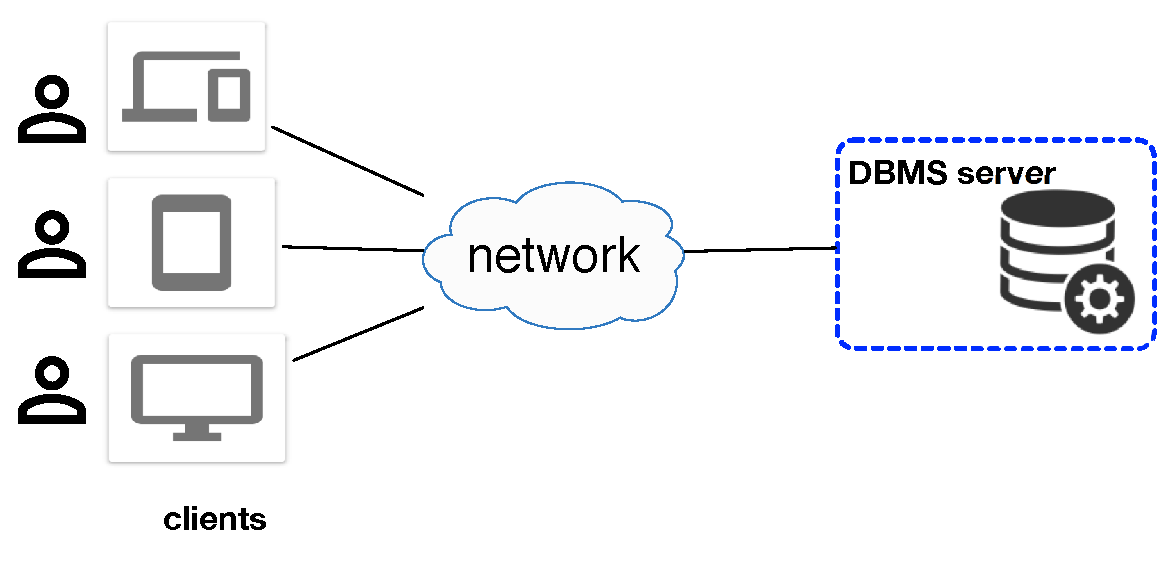
\includegraphics[width=1.25\textwidth]{figures/client_server_cloud}
\end{column}
\end{columns}

\vskip0.5em

Other implications:
\begin{enumerate}[label=(\arabic*)]
\item \underline{scaling} to more users means buying a bigger server
\item all data input/output flows through the \underline{network}
\end{enumerate}
 
This model is best for centralized applications where the provider is responsible for the data (e.g., universities, banks, government agencies, etc.) \textbf{and} where Internet connectivity is a given.

\end{frame}


%
% ---------------------------------------------------------------------------
%
\begin{frame}{Client-Server with DBMS API}

Application developers can use APIs to connect to the DBMS via the network.

\vskip1em

\begin{center}
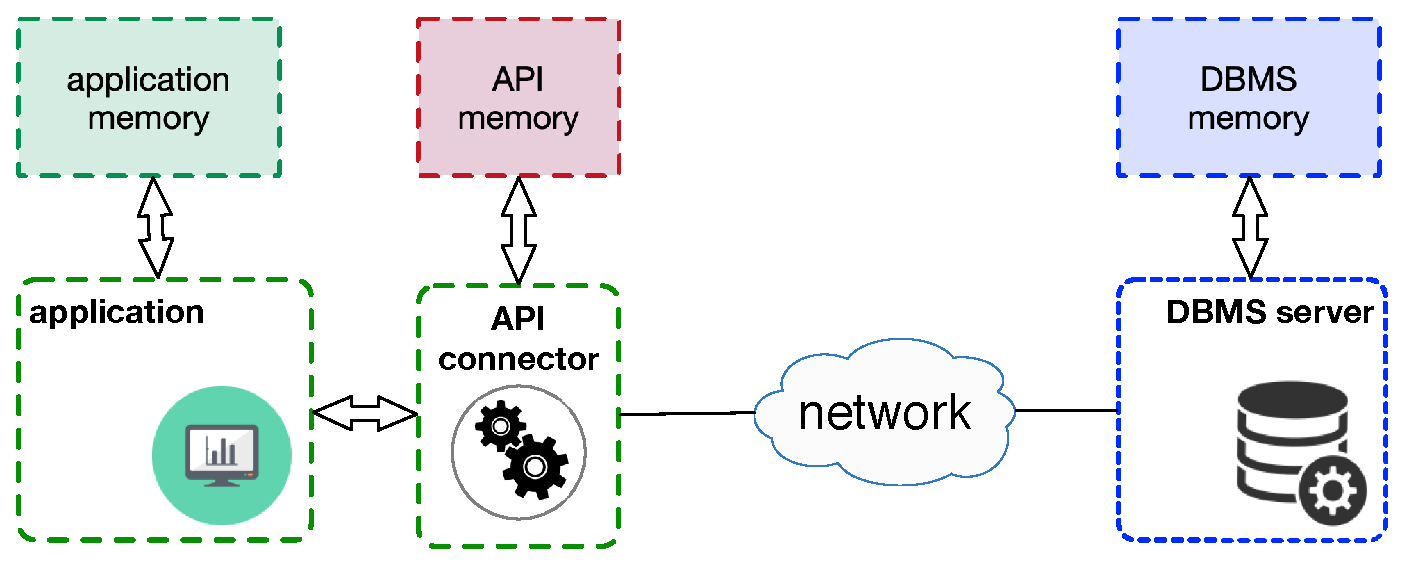
\includegraphics[width=0.6\textwidth]{figures/client_server_API.eps}
\end{center}

\vskip1em

ODBC\footnote{\url{https://en.wikipedia.org/wiki/Open_Database_Connectivity}} (Open Database Connectivity) is an industry standard supported by many languages and DBMS vendors.

\end{frame}


%
% ---------------------------------------------------------------------------
%
\begin{frame}{Client-Server with Embedded SQL}

A more efficient way to deploy a client-server application is to \textbf{embed}\footnote{\url{https://en.wikipedia.org/wiki/Embedded_SQL}} the libraries for connecting to the DBMS within the application itself.

\vskip1em

\begin{center}
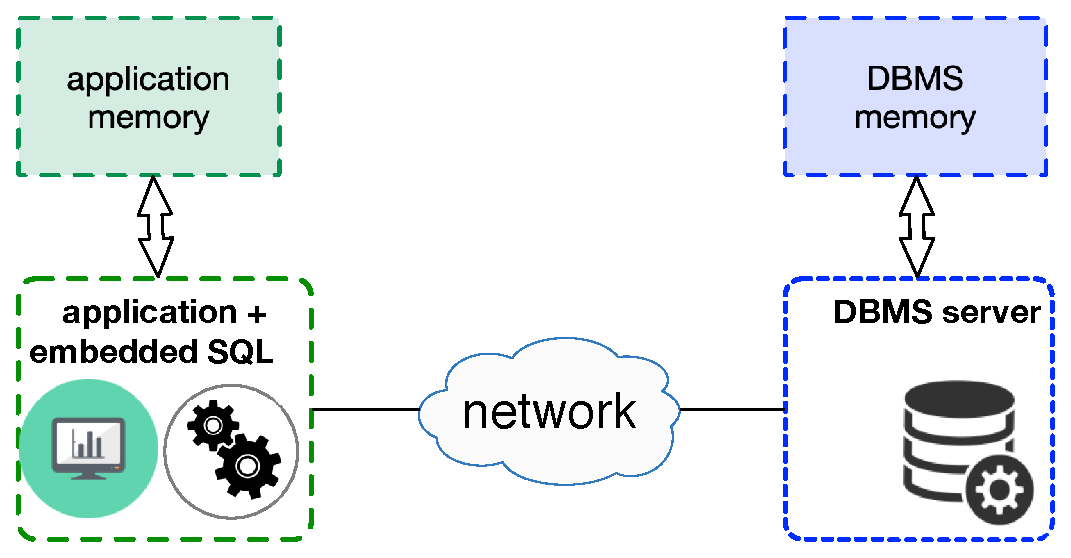
\includegraphics[width=0.6\textwidth]{figures/embedded_SQL_client_server.eps}
\end{center}

\vskip1em

This is done by \textbf{compiling} the application and the libraries together.

\end{frame}


%
% ---------------------------------------------------------------------------
%
\begin{frame}{Client-Server on the same device}

DBMSs are being deployed more and more for \textbf{single-user} applications, e.g., mobile apps or games.

A simple (\alert{but inefficient}) way to do that is to use the standard client-server architecture where both execute as separate processes on the same device:

\vskip1em

\begin{center}
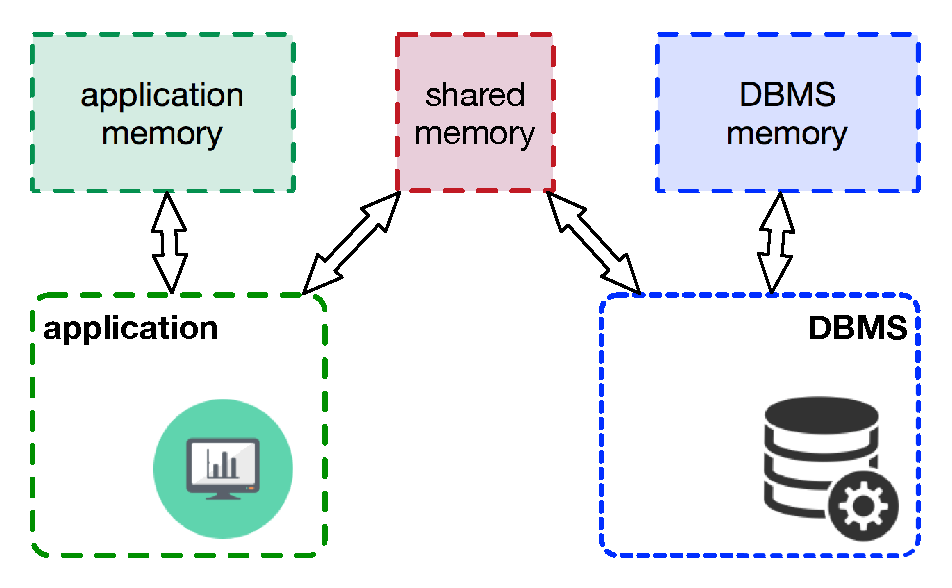
\includegraphics[width=0.6\textwidth]{figures/API_local_system.eps}
\end{center}
\end{frame}



%
% ---------------------------------------------------------------------------
%
\begin{frame}
\vskip2em
\begin{columns}
\begin{column}{0.6\textwidth}

What is so bad about this?

\end{column}
\begin{column}{0.3124\textwidth}
\hspace*{-3.5em}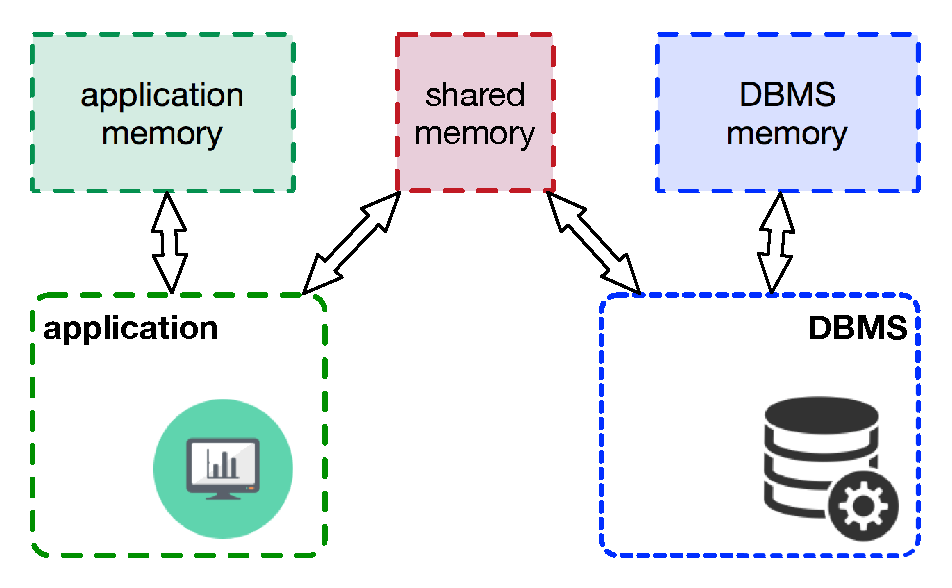
\includegraphics[width=1.25\textwidth]{figures/API_local_system.eps}
\end{column}
\end{columns}

\vskip0.5em

Data must be copied multiple times:\\
 - from storage to DBMS buffers (and back)\\
 - from DBMS buffers to shared pages in memory\footnote{One of the best ways of implementing inter-process communication... Read up \url{https://en.wikipedia.org/wiki/Inter-process_communication}} (and back)\\
 - from shared pages to the application (and back)

This is not only wasteful but also \underline{much slower}:\\
 - even if the computer is \emph{over-provisioned} 

\end{frame}


%
% ---------------------------------------------------------------------------
%
\begin{frame}{Embedded DBMS}

The right way of deploying single-user applications that need DBMS support is to \textbf{embed} the DBMS code inside the application:

\begin{center}
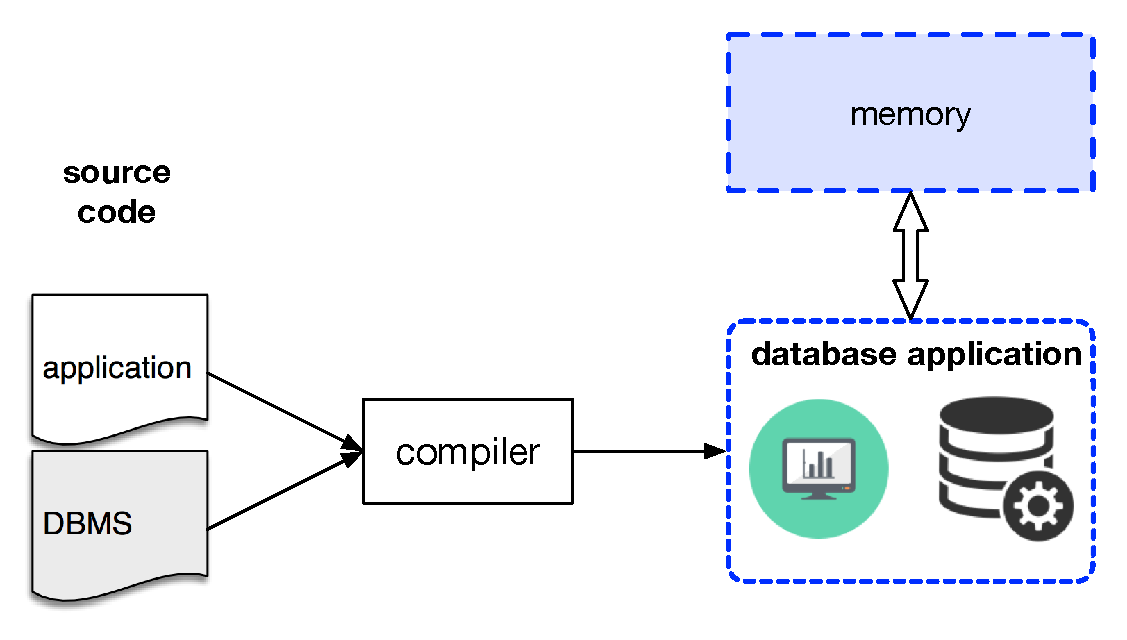
\includegraphics[width=0.6\textwidth]{figures/embedded_dbms_code.eps}
\end{center}

SQLite was designed to be embedded in applications in ANSI C.\footnote{\url{https://sqlite.org/cintro.html}}

\end{frame}


%
% ---------------------------------------------------------------------------
%
\begin{frame}
\vskip2em
\begin{columns}
\begin{column}{0.6\textwidth}

What is so good about this?

\end{column}
\begin{column}{0.3124\textwidth}
\hspace*{-3.5em}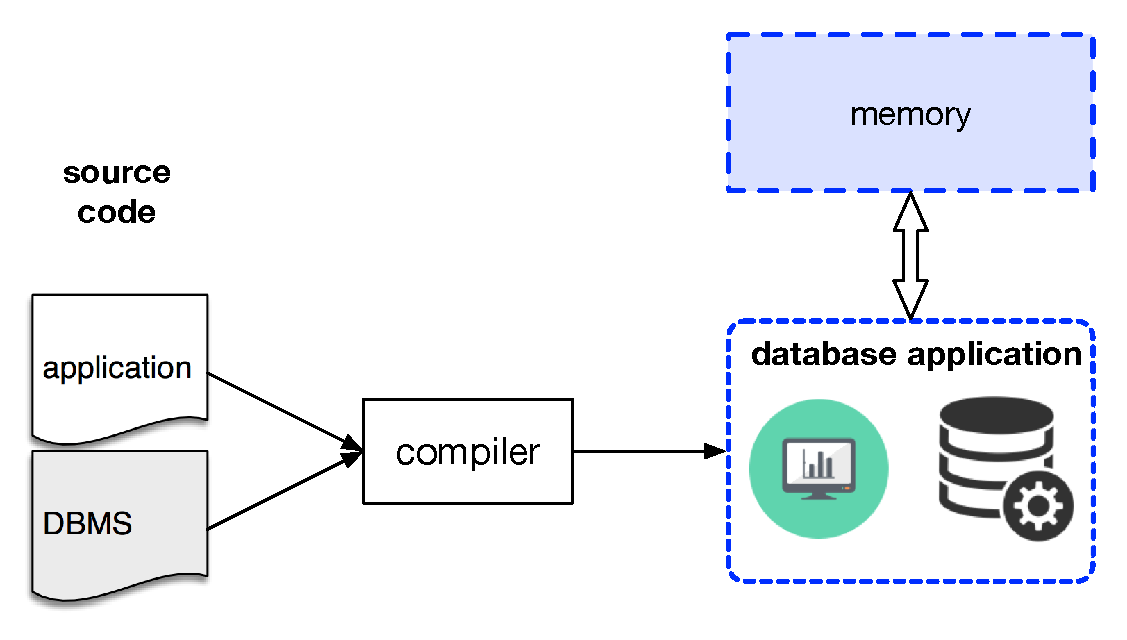
\includegraphics[width=1.25\textwidth]{figures/embedded_dbms_code.eps}
\end{column}
\end{columns}

\vskip0.5em

No copying data around: ``DBMS'' buffers are easily accessible by the ``application''.

Unused/unnecessary components of the DBMS are not compiled into the application, resulting in code with a smaller footprint.

\vskip1em

Embedded data management is a strong trend with mobile apps, computer games, web browsers, etc.

\end{frame}

%
% ---------------------------------------------------------------------------
%
\begin{frame}{ASIDE: embedded SQL in the wild}

Compiling SQL into native code?\\
 - although still a research topic, this is not mad science!\\
 - will be mainstream pretty soon.

Because of its small footprint, efficiency, main-memory option, and its public domain license, SQLite is probably the \textbf{most widely used} relational DBMS in the world today.

Modern MMORPG computer games comprise worlds with thousands of objects which are related in complex ways. Many of them already use relational DBMSs in a client-server mode, and some are moving to an embedded mode.

\end{frame}


%
%
% Further reading/other DBMSs
%
%

%
% ---------------------------------------------------------------------------
%
\begin{frame}{Further references/resources}

Other in-memory/main-memory databases besides SQLite:
\small{\url{https://en.wikipedia.org/wiki/List_of_in-memory_databases}}

\vskip1em

PostgreSQL is an open-source, enterprise-scale client-server DBMSs:
\small{\url{https://www.postgresql.org}}

\vskip1em

Apache Derby is an open-source relational DBMS written in and for Java. It can be efficiently embedded inside Java applications:
\small{\url{http://db.apache.org/derby/}}

\end{frame}
